\section{System's Perspective}

\todo{Refferences?}
\subsection{Design \& Architecture}
Frontend is built using Next.js\cite{nextjs}. The data is fetched through a Go Gin\cite{gin-gonic} API interacting with the database through an ORM called GORM\cite{gorm}. The service is deployed through Docker with the backend and frontend being separate containers. To provide insights into the system we also deploy "supporting" containers like EFK stack, Grafana \& Prometheus. Finally, we also have a container for Nginx responsible for providing a network configuration that allows us to have an SSL certificate along with a domain address.
\\\\
We chose Digital Ocean as our hosting provider using their VM service "Droplets". The system consists of 3 droplets, 1 manager node, and 2 worker nodes working together in a docker swarm setup \todo{Make sure we actually do this before turnin}. We also pay for a hosted postgres database on Digital Ocean that we use to store all messages, follower relations and users. 

\begin{figure}[h!]
    \centering
    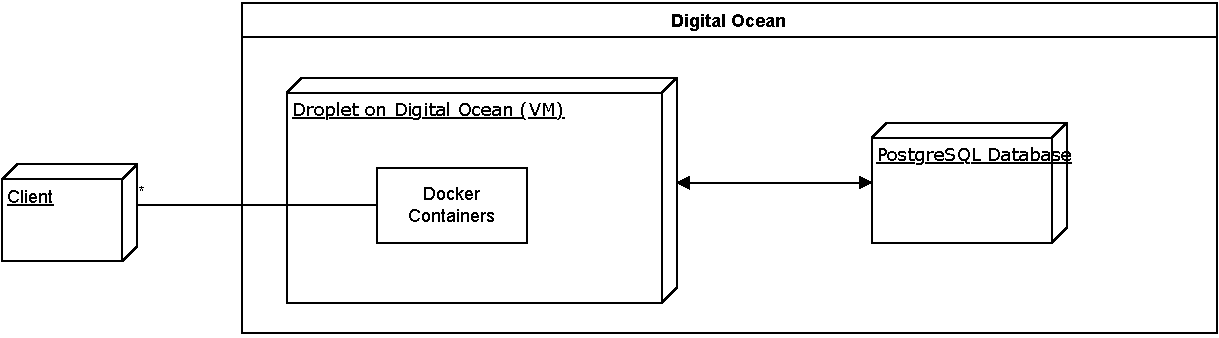
\includegraphics[scale=0.6]{diagrams/infrastructure.pdf}
    \caption{Digital Ocean infrastructure}
    \label{fig:do_infrastructure}
\end{figure}
\todo{If we do swarm, then update image}

\subsection{Dependencies on all levels of abstraction}
\textbf{Hosting} depends on Virtual Machines (droplets) \& Database(postgres) managed by DigitalOcean. 
\\\\
\textbf{CI/CD chain} depends on Github Actions as a service Github runs. 
\\\\
\textbf{Remote code repository} is hosted on Github.
\\\\
\textbf{Project dependencies:} Both the frontend and backend solutions rely on external dependencies and libraries in order to work. It is not feasible to construct every single package from the ground up, which is why we chose this approach. Since the frontend is build using Next.js we use npm as a package manager, which constructs a "package.json" that handles the dependencies. For the go backend, we also rely on external packages, that are all stored in a "go.mod" file. Both the "package.json" (\ref{subsec:package.json}) and "go.mod" (\ref{subsec:go.mod}) can be seen in the appendix.

\subsection{Important interactions of subsystems}
\todo{wtf here}
\subsection{Current state of system}
% describe result of static analyis
SonarCloud result: \url{https://sonarcloud.io/project/overview?id=DevOps-CI-CDont_DevOps-CI-CDont2}
\begin{enumerate}
    \item 1 bug ("an unnecessary expression in an if statement")
    \item 0 vulnerabilities
    \item 51 code smells (naming convention breaches, some things could be constants)
    \item 11 Security hotspots (eg. secrets in docker environment variables)
\end{enumerate}

\subsection{License \& compatibility with direct dependencies}
% not sure how to check this

\subsection{Weekly Tasks}
The weekly tasked, were based on the exercises that were given in the lecture.

\subsection{Choice of technologies}
\subsubsection{Frontend}
We chose Next.js as our frontend service, due to it's many build in features, such as:

\begin{enumerate}
    \item - Code splitting
    \item - Routing support
    \item- Server Side Rendering
    \item- Layouts and Components
    \item- API routes
    \item- Build in optimizations
    \item- Support for middleware
\end{enumerate}
Furthermore, we have added Tailwindcss as a CSS utility class for easy styling.
Having Server Side Rendering (SSR) isn't necessary for the Minitwit application, but it allows us to fetch data and build a page on the server, which gives a much better score on Google Lighthouse and also removes Cumulative Layout Shift (CLS), which gives a better user experience.

Having code splitting, divides the js build files into smaller files, making the size smaller and therefore 'lighter' to fetch (Making the application faster).

Next.js handles routing and API routes in the pages directory (Next.js 13 = app directory). This removes the overhead of having to create a react router that points to the different page components. Having a dedicated API routes folder, allows us to create API routes, that can fetch our backend data with ease. The API routes folder removes many issues and privacy related data, such as enviornment variables.

The Minitwit application has a user authentication system. With Next.js we can create a middleware that removes unauthenticated users from accessing pages, they're not allowed to view.
\subsubsection{API technology choice}
We chose to use Go with Gin to make a RESTful API because:
It is a new language for all group members, so we can learn it together. We thought it would be an interesting language to build an API in. It is a pretty modern language, that is said to be built for concurrency, it's fast.  
*"The story goes that Google engineers designed Go while waiting for other programs to compile. Their frustration at their toolset forced them to rethink system programming from the ground up, creating a lean, mean, and compiled solution that allows for massive multithreading, concurrency, and performance under pressure."* - <https://stackoverflow.blog/2020/11/02/go-golang-learn-fast-programming-languages/>
We first expected to use Go with Gorilla Mux, but we found out that that library has been archived - and so decided not to use Mux.
\subsubsection{Database}
At first we "inherited a local" database setup (a db file inside backend/tmp), and we didn't change that when we started containerizing the application. This was a very bad setup for real production data, as the database would be lost when the container was restarted. \\
We have since changed the database to a hosted PostgreSQL database via DigitalOcean.
\subsubsection{Domain}
We used Name.com to purchase \url{cicdont.live} for a year, for free.

\todo{Skal der være flere technology choices her?
"MSc students remember to argue for the choice of technologies and decisions for at least all cases for which we asked you to do so in the tasks at the end of each session."}